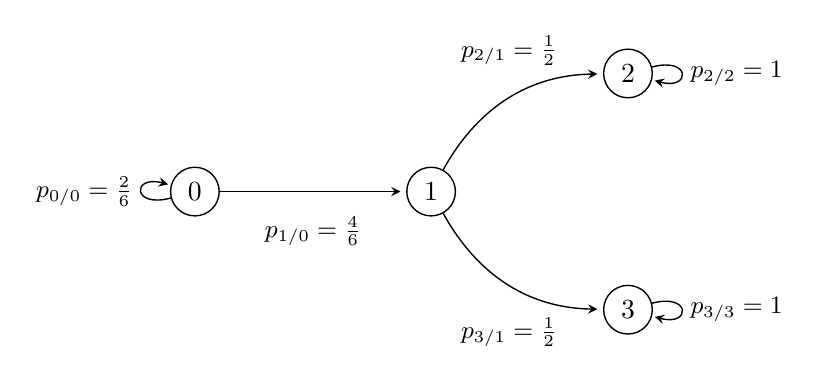
\begin{tikzpicture}[->, >= stealth, shorten >=2pt , line width =0.5 pt, node distance =2 cm]//
\node [circle, draw] (0) at (0, 1.5) {$0$};
  \node [circle, draw] (1) at (3, 1.5) {$1$};
  \node [circle, draw] (2) at (5.5, 3) {$2$};
  \node [circle, draw] (3) at (5.5, 0) {$3$};
  
  \begin{small}
    \path (0) edge [loop left] node [left] {$p_{0/0} = \frac{2}{6}$} (0);
    \path (0) edge node [below = 0.2cm] {$p_{1/0} = \frac{4}{6}$} (1);
  
    \path (1) edge [bend left] node [above = 0.3cm] {$p_{2/1} = \frac{1}{2}$} (2);
    \path (1) edge [bend right] node [below = 0.3cm] {$p_{3/1} = \frac{1}{2}$} (3);
  
    \path (2) edge [loop right] node {$p_{2/2} = 1$} (2);
    \path (3) edge [loop right] node {$p_{3/3} = 1$} (3);
  \end{small}
        \end{tikzpicture}
